% arara: pdflatex: { interaction : nonstopmode }
% arara: biber: { options: ['--isbn-normalise'] }

\documentclass[
  t,% place content on top of the page
]{_style/tudelft-beamerposter}

\usepackage[
  orientation=portrait,
  size=a2,
  scale=1.45, % scaling factor to make sure the page looks full
]{beamerposter}

\usepackage{ragged2e}

\makeatletter % without this, the color name 'beamer@tcb@titlebg' would be inaccessible.
\tcbset{
  % optionally: a border around the 'blocks', in the color of the title background:
  borderline={1.5pt}{0pt}{beamer@tcb@titlebg},
}
\makeatother

% used for headers, blocks etc.
\setbeamercolor{bars}{bg=tud primary, fg=white}

\addbibresource{bibfile.bib}

\title[title]{Comparing Crop Types in Different Regions of Germany Using High Resolution Remote Sensing Imagery and Random Forest Classification}
\author[Brand \& Lehmann \& Menezes]{T.~Brand \and T.~Lehmann \and L.~Menezes \and University of Münster}

\setlength{\columnsep}{0.1\linewidth}

\setlength{\TPHorizModule}{\paperwidth}
\setlength{\TPVertModule}{\paperheight}

\newcommand{\footertext}{%
  \ifleftfooterwhite%
    \textcolor{white}{\tudlogo\,\descriptor}%
  \else%
    \tudlogo[tud topaz]\,\descriptor%
  \fi%
}

\setbeamertemplate{footline}{\Huge\quad\raisebox{1.4ex}{\footertext}}

% Keep inside the main file, since probably the size, etc. has to be changed
% for every individual poster
% https://www.overleaf.com/learn/latex/Font_sizes%2C_families%2C_and_styles
\renewcommand\maketitle{
  {\begin{beamercolorbox}[
    wd=\paperwidth,
  ]{bars}{%
    \centering\robotoslab%
    \vskip0.01\paperheight
    \begin{minipage}{\textwidth-30mm}\centering
      \Huge\inserttitle\\[0.01\paperheight]
      %  \hspace*{10mm} % throw in some more logo's, if you need to...
      %  \includegraphics[width=45mm]{icons/buildings/TU Delft - icon - AULA.pdf}\hfill
      %  \includegraphics[width=45mm]{icons/buildings/LIB.pdf}\hfill
      %\begin{minipage}{\textwidth-150mm}\centering
      \LARGE\insertsubtitle\\[0.01\paperheight]
      \insertauthor\\[0.01\paperheight]
      \normalsize\insertinstitute\\[0.01\paperheight]
      %\end{minipage}\hfill
      % \includegraphics[width=45mm]{icons/communication/conference.pdf}\hfill
      % \includegraphics[width=45mm]{icons/general/puzzle.pdf}
      % \hspace*{10mm}
    \end{minipage}\\
    \vskip0.01\paperheight
  }\end{beamercolorbox}}%
}

\usepackage{endnotes}
\let\footnote=\endnote

\begin{document}

\begin{frame}
  \maketitle

  \begin{columns}[onlytextwidth, T]
    \begin{column}{\widthfrac{2}{3}}
        \begin{columns}[T]
            \begin{column}{\widthfrac{1}{2}}
            
              \section*{Abstract}
              \justifying
               Crop classification using remote sensing data is crucial for agricultural management and monitoring. It would also emphasize the challenges posed by intra-class variability and the potential of combined spectral and temporal data for improved accuracy, particularly in large-scale applications. 
              
              \section*{Objectives}
              \justifying
              The objective of this study is to classify the crops in the selected area of interest by using Random Forest and Texture Analysis. The results are then compared with different regions to evaluate the variety in crop types.
            \end{column}
            
            \begin{column}{\widthfrac{1}{2}}
                \begin{figure}
                    \begin{center}
                        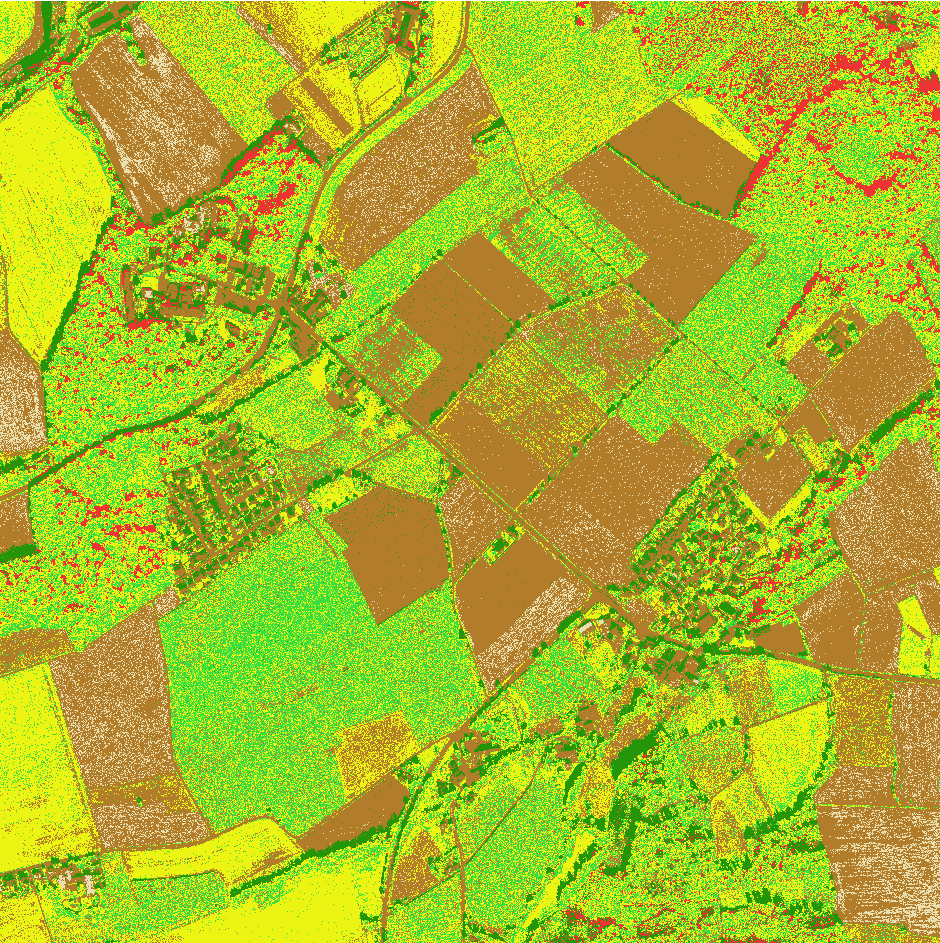
\includegraphics[scale=0.45]{graphs/textureAndColour2x2wickede.png}
                        \caption{Wickede, RGB and Texture 2x2 Tiles}
                        \label{fig:topCenter}
                    \end{center}     
                \end{figure}
                         
            \end{column}
        \end{columns}
        
      \section*{Methodology}
      \begin{block}{Constraints}
        \begin{itemize}
          \item Data from two regions with different typical crops
          \item Municipalities Laer (Münster) and Wickede (Arnsberg/ Soest)
          \item No-Code approach with QGIS and Orfeo Toolbox (OTB)
        \end{itemize}
      \end{block}
      
      \begin{block}{Image Processing}
        \begin{itemize}
          \item Digital orthophotos (DOP) from NRW in TIFF format
          \item Texture feature extraction using Orfeo Toolbox standard tools (Haralick Texture Extraction)
          \item Manually labeled training polygons
          \item Random Forest classification
          \SubItem Trained on RGB imagery and texture features \cite{rs70101074}
        \end{itemize}
      \end{block}

      \begin{multicols}{2}
        \begin{block}{Classes}
          \begin{itemize}
            \item Bare Soil
            \item Grassland
            \item Corn
            \item Cereal
            \item Potatoes
            \item Woods
          \end{itemize}
          \vspace{1.25cm}
        \end{block}

        \begin{block}{Statistics}
            \begin{itemize}
                \item To compare different regions, one simple and naive approach is counting classified pixels. 
                \item Another extending approach is calculating the total area from the counted/ classified pixels.
                \item Calculated with QGIS Raster Unique Value Report
            \end{itemize}
        \end{block}
      \end{multicols}

      \section*{Visualisation}
        \begin{figure}[h!]
            \begin{minipage}{.5\textwidth}
                \centering
                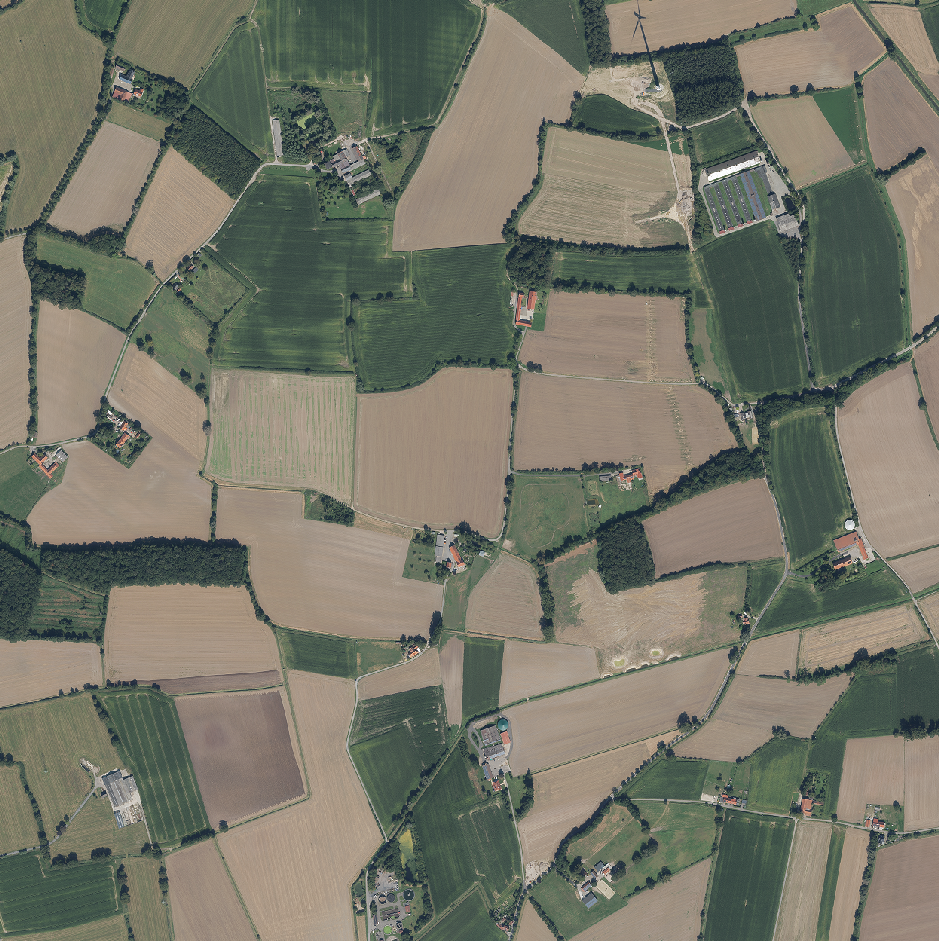
\includegraphics[scale=0.45]{graphs/dop2x2laer.png}
                \caption{Laer, DOP 2x2 Tiles}
                \label{fig:sub1}
            \end{minipage}%
            \begin{minipage}{.5\textwidth}
                \centering
                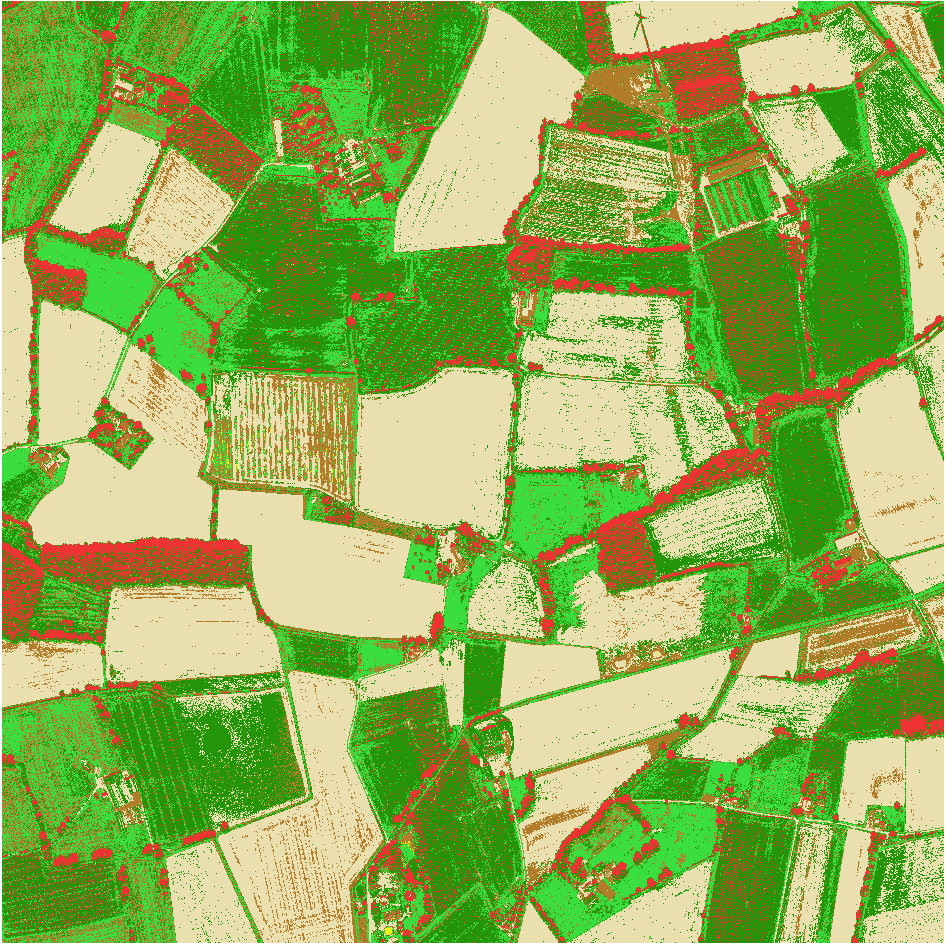
\includegraphics[scale=0.45]{graphs/iteration2x2laer.png}
                \caption{Laer, only RGB 2x2 Tiles}
                \label{fig:enter-label}
            \end{minipage}%
            \begin{minipage}{.5\textwidth}
                \centering
                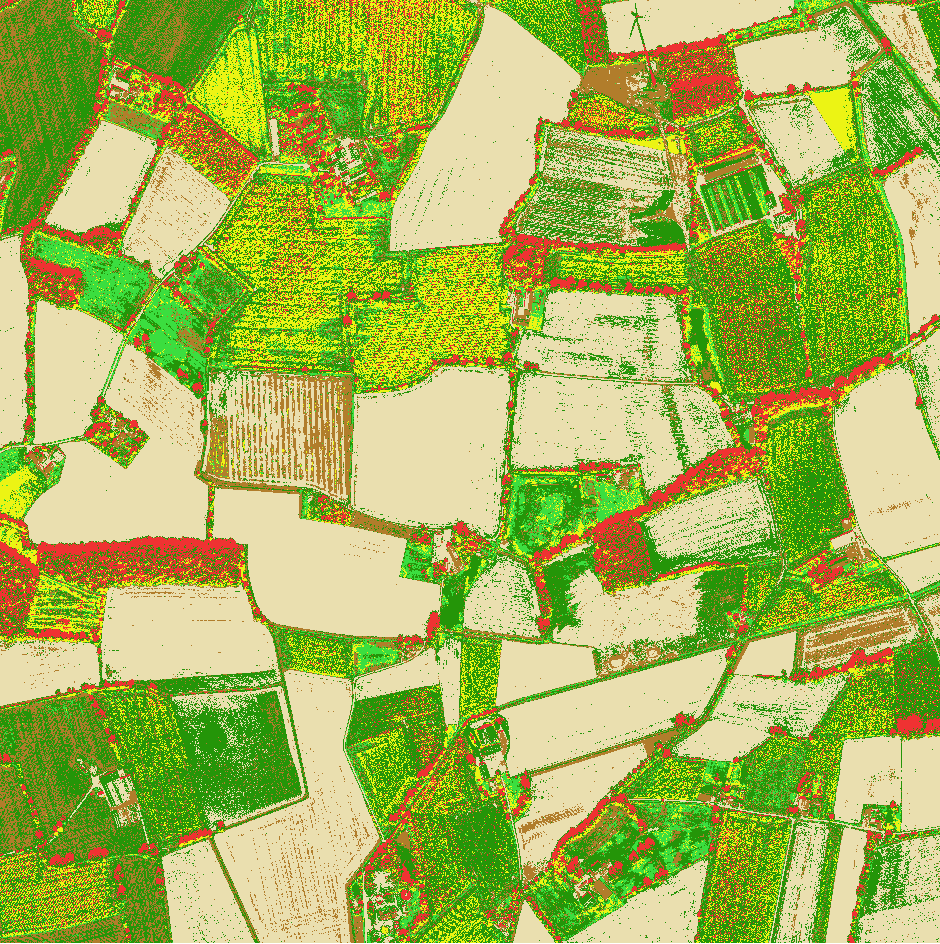
\includegraphics[scale=0.45]{graphs/textureAndColour2x2laer.png}
                \caption{Laer, RGB and Texture 2x2 Tiles}
                \label{fig:enter-label}
            \end{minipage}%
        \end{figure}

    \end{column}
    \begin{column}{\widthfrac{1}{3}}
      \section*{Results}
      \justifying
      The Random Forest classification successfully distinguished crop types across both regions. Laer shows dominant corn cultivation (1159 ha) and bare soil (1567 ha), while Wickede is characterized by extensive potato farming (1423 ha) and higher grassland coverage (767 ha), demonstrating clear regional agricultural differences. But it needs to be said that the results are not perfect and future improvements are needed.

      \section*{Legend}
      \begin{figure}
        \centering
        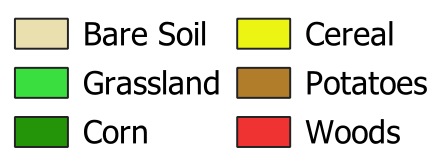
\includegraphics[width=1\linewidth]{graphs/legend.png}
        \label{fig:legend}
      \end{figure}

     
  
      \AtNextBibliography{\normalsize}% or in the preamble \AtBeginBibliography{\small}
      \printbibliography

      \vspace{1cm}
        
      \section*{GitHub}
      \justifying
        A digital version of this presentation can be found here:
      \url{https://github.com/tlehman1/AOHRSI_CropDetechtion}.
      \\ Here is a QR code for GitHub:
  
      \begin{center}
        \qrcode[height=3cm]{https://github.com/tlehman1/AOHRSI_CropDetechtion}
      \end{center}
    \end{column}
  \end{columns}
\end{frame}

\end{document}
